% ============================================================
% 中文信息学报 venue profile（jcip）受限验证合成样稿（编号一致性版）
% 合成内容，不代表真实论文；只使用 profile.supported_commands 内的命令。
% 引用一律走 refs.bib（profile 要求，不用 thebibliography）。
% 覆盖：3 公式（前向/后向/重复引用）、2 图、2 表、多文件 input 对象。
% ============================================================
\documentclass[10pt,twocolumn]{article}
\usepackage{ctex}
\usepackage{amsmath,amssymb}
\usepackage{graphicx}
\usepackage{booktabs}
\usepackage[numbers]{natbib}
\usepackage[affil-it]{authblk}

\title{面向合成验证的中英混合文本转换链路评估方法}
\author{张三$^{1}$ \and 李四$^{1,2}$}
\affil{$^{1}$示例大学计算机学院，北京 100000 \and $^{2}$示例研究院人工智能实验室，上海 200000}

\begin{document}
\maketitle

\begin{abstract}
本文提出一种面向合成验证的中英混合文本转换链路评估方法。文中式~\eqref{eq:gain}
与图~\ref{fig:gain} 为前向引用（对象在其后出现），式~\eqref{eq:attn} 与
表~\ref{tab:params} 为后向引用，式~\eqref{eq:attn} 被重复引用以验证多次
引用一致性。本文不构成真实研究成果。
\end{abstract}

\noindent\textbf{关键词：}转换链路；合成验证；中英混合

\noindent\textbf{Evaluation of Conversion Pipelines for Code-Switched Text (Synthetic)}
\vspace{0.5em}

\noindent This synthetic study evaluates a constrained conversion pipeline
covering forward/backward/repeated references over equations, figures and tables.

\section{引言}\label{sec:intro}

中英混合场景（code-switching）给文本处理带来词表与语义对齐的双重挑战
\cite{zhang2025}。现有评估方法 \cite{smith2024} 通常将两类文本分开建模。
本文的贡献如下：

\begin{itemize}
  \item 提出融合注意力权重的示例评估模型；
  \item 在合成数据上验证其相对基线的提升；
  \item 给出可复现的受限导出验证路径。
\end{itemize}

\section{方法}\label{sec:method}

\subsection{注意力机制}

编码器输出 $h_{t}$ 与注意力权重 $\alpha_{t}$ 的计算如式~\eqref{eq:attn}
所示：

\begin{equation}
  \alpha_{t} = \frac{\exp(\boldsymbol{w}^{\top}\boldsymbol{h}_{t})}
                   {\sum_{k=1}^{T}\exp(\boldsymbol{w}^{\top}\boldsymbol{h}_{k})}
  \label{eq:attn}
\end{equation}

其中 $T$ 为序列长度，$\boldsymbol{w}$ 为可学习的打分向量。融合增益由
式~\eqref{eq:gain} 给出（该式在下一节定义，用于验证前向引用）：

\begin{equation}
  g = 1 - \prod_{k=1}^{K}(1-\alpha_{k})
  \label{eq:gain}
\end{equation}

\subsection{训练设置与多文件对象}

训练使用的主要超参数见表~\ref{tab:params}；对比配置见表~\ref{tab:cmp}。

\begin{table}[htbp]
  \centering
  \caption{训练超参数（合成示例）}
  \label{tab:params}
  \begin{tabular}{lll}
    \toprule
    参数 & 取值 & 说明 \\
    \midrule
    学习率 & 3e-5 & AdamW 优化器 \\
    批大小 & 32 & 单卡训练 \\
    训练轮数 & 10 & 验证集早停 \\
    \bottomrule
  \end{tabular}
\end{table}

\begin{table}[htbp]
  \centering
  \caption{对比配置（合成示例）}
  \label{tab:cmp}
  \begin{tabular}{ll}
    \toprule
    配置 & 值 \\
    \midrule
    优化器 & AdamW \\
    调度 & cosine \\
    \bottomrule
  \end{tabular}
\end{table}

来自被 \texttt{input} 子文件的公式如式~\eqref{eq:part} 所示
（验证多文件工程中的对象编号）：
\begin{equation}
  p = \frac{n_{p}}{n}
  \label{eq:part}
\end{equation}


\section{结果}

\begin{figure}[htbp]
  \centering
  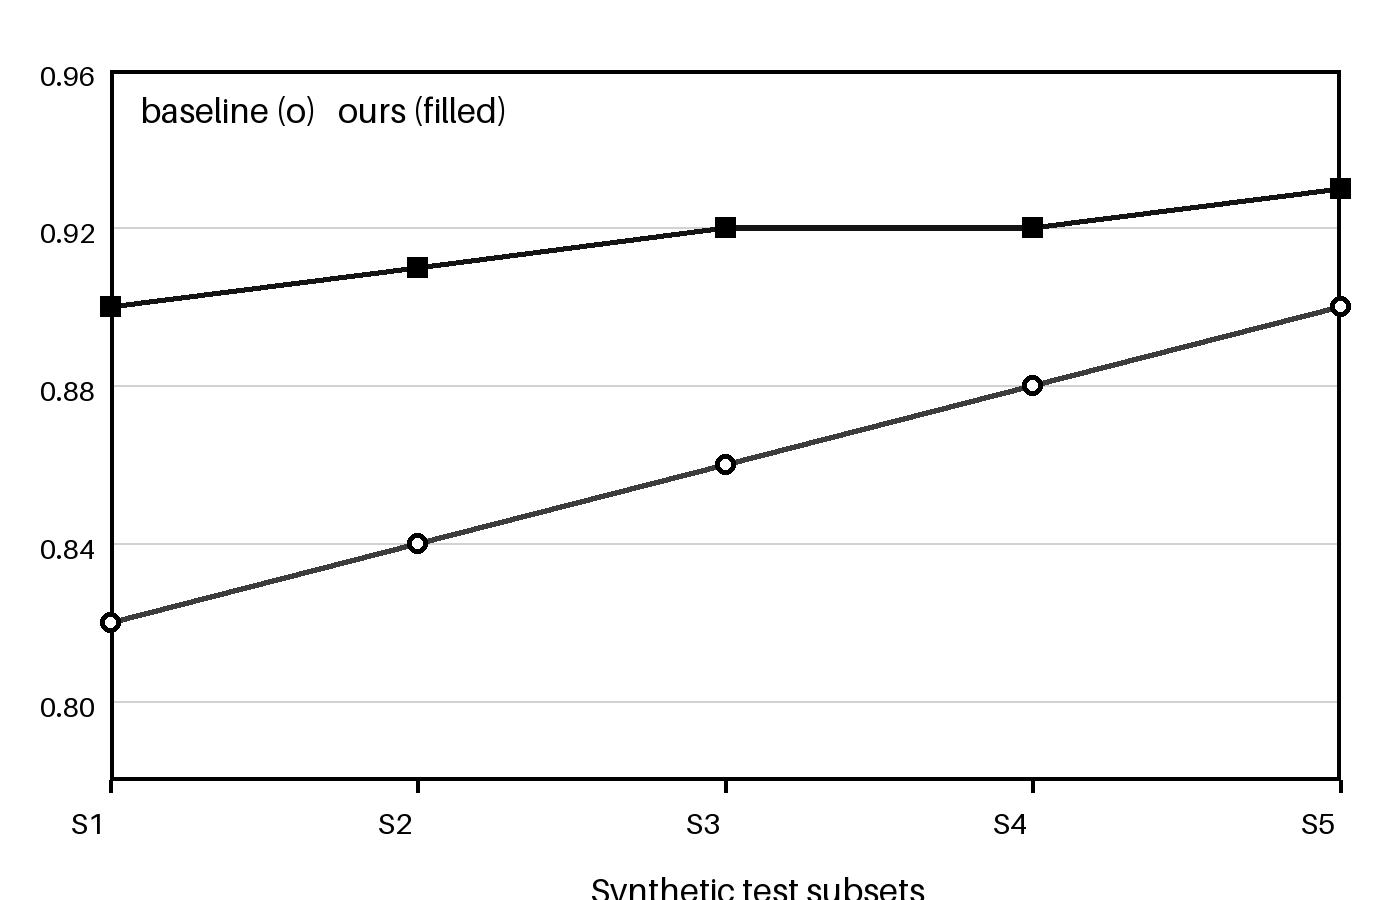
\includegraphics[width=\linewidth]{fig1.png}
  \caption{两组方法在测试集上的准确率对比（合成数据）}
  \label{fig:acc}
\end{figure}

如图~\ref{fig:acc} 所示，所提方法在五个合成测试子集上的准确率均高于
基线。融合机制的额外收益见图~\ref{fig:gain}
（前向引用，对象定义见下）。

\begin{figure}[htbp]
  \centering
  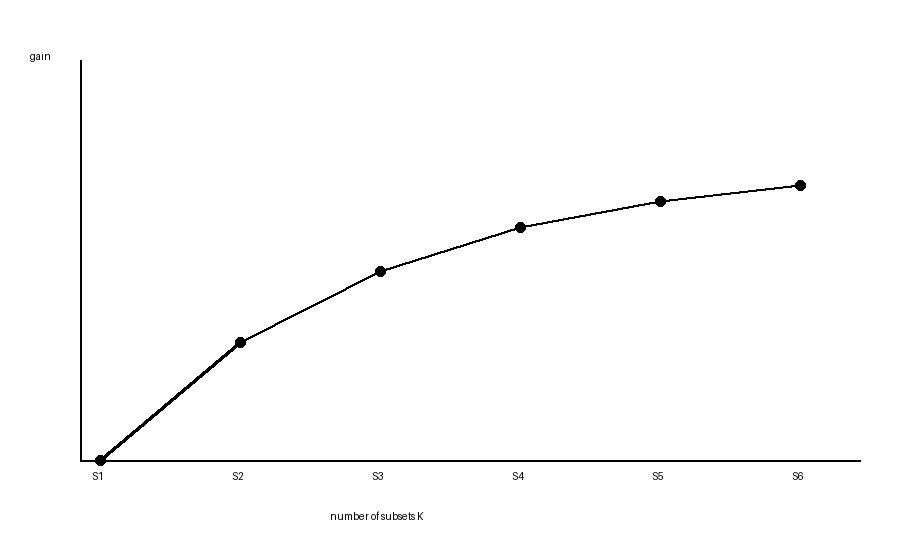
\includegraphics[width=\linewidth]{fig2.png}
  \caption{融合增益随子集数变化（合成数据）}
  \label{fig:gain}
\end{figure}

\section{结论}

本文为合成验证样稿，实验结论不构成真实研究成果。注意力机制的示例
实现见式~\eqref{eq:attn}，融合增益见式~\eqref{eq:gain}，多文件公式见
式~\eqref{eq:part}。

\bibliographystyle{unsrtnat}
\bibliography{refs}

\end{document}
